\subsection{Instrumentation}

Similar to any other run time monitoring systems, RPTR needs to perform instrumentation before the launch of the targeting system in order to keep track of the interesting information about the program execution. In particular, we are to instrument the eight ROS API calls. These eight functions include all the function variants in ROS that interacts with parameters. Although only three actions are performed, ROS provides two variants of each: a �bare� version and a �handle� version. In addition, there are four variants for getting the value of a parameter. The difference between the bare and the handle version is the namespace they access. Accessing a parameter via the bare API call will be resolved relative to the node�s namespace. Accessing a parameter with the handle API call will be resolved relative to the node handle�s namespace (which is specified when the node handle is created). See Fig.~\ref{fig:ParamMethods} for a listing of these calls.
 
\begin{figure}
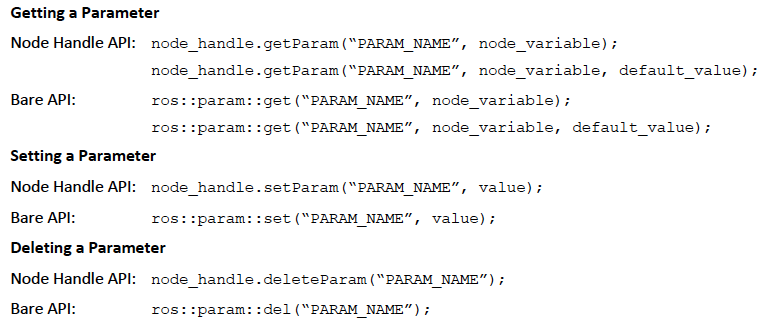
\includegraphics[scale=0.5]{images/ParamMethods}
\caption{Parameter Methods of Interest}
\label{fig:ParamMethods}
\end{figure}
 
The purpose of the instrumentation is to collect the parameter usage along the whole execution process of the program, changes being made or values being set, etc. The easiest way to perform the instrumentation is to write up eight method calls in a RPTR library, with each corresponding to a ROS API call. In the RPTR library functions, we first extract information from the original calls, publish the information to our destination and then execute the original API calls. In the fashion, we make the minimal changes to the code by replacing one function with another and introducing another library for the system.
 
Concerning the specifics of instrumentation, our most promising option first started with an AOP approach using AspectC++. Code that calls a piece of RPTR will be instrumented before, around, during or after each of the API calls listed in Figure 2.1, as well as after the creation of a node handle. According to the AspectC++ documentation, we have access to all context information from each of the function calls, including the value of arguments. Therefore, we thought we could instrument aspects based on specific function signatures and could access to the values of their arguments as well as which node executed the request, we would have enough information to dynamically store everything required for our analysis.  Everything came together for this approach until we found out that AspectC++ does not support multi-threaded programs, which is one of the key features in ROS systems.
 
Inspired by the AspectC++ approach where aspects are instrumented based on comparison with the specific function signatures, we perform the instrumentation based on the matching the function signature. We developed a set of regular expressions for each of the eight functions of interest. One match with the regular expression indicates a function interacting with parameters, and we need to replace this match with the RPTR function that publishes the parameter information and also execute the ROS API functionality. Based on this understanding of instrumentation, RPTR instrumentor first starts with a launch file, extracts all the nodes that it involves in the launch, then iterates through all the nodes to find all the cpp files, performs the regular expression matching and finally instruments the system. The instrumentation includes 4 steps: (1) replace the ROS API function with RPTR library function, (2) add the dependence on RPTRLibInterface, (3) \#include <RPTRLibInterface.h> in the cpp file, (4) add a global variable of type RPTR. Note the point that we are not instrumenting the header files. This would cause us to possibly lose information about the parameters. However, we believe this is a legitimate limitation. We started with instrumenting both cpp files and the header files. However, the problem is that we need to introduce a global variable in the file that may reference the RPTR library. If we introduce one variable in the header file, and this header file is included by multiple cpp files in the system, the compiler complains about multiple definition of the same type. There is basically no way of getting around this if we want to instrument the header files.
 
We did notice the possible limitation of this instrumentation approach. First, based on text processing and regular expression matching, we process the source code line by line. It is very likely that the function can be written into multiple lines in the code, which would cause the instrumentation to miss this possible match. Second, the defined macros make the matching even more difficult, as the function call would not follow the strict regular expression for matching.
 
To make the approach more compact, we could perform a second layer of validation after the instrumentation on the object files. At first, we proposed to validate using the �grep� command. However, when we were evaluating this validation approach, we realized that grep command still works with each line of the source code, which introduce the risk of missing matches again. Also, it is hard to decide on what to grep for, especially taking into consideration about macro concatenation. Take one ROS API function as an example, �ros::param::get(�param\_name� ,  variable)�. This function makes it hard to decide what to grep for, as �ros�, �param�, �get� can all get into different lines and just perform �grep param� generates a lot more results that are not related to the function. However, we do not have these ambiguities if we perform the second layer of validation on the object file after compilation. On the object level, first all the macros are compiled, and all the functions are named. For example, the bare API �ros::param:get� will have a mangling name that we can grep for. We only need to validate whether these functions are only called from the RPTR library and no where else in the ROS system. For other node handle API, we can grep the keyword �getParam, setParam, delParam� to make sure they are not called from the ROS nodes. This second step of the validation is actually precise information that we can present to the user. Also, what we need to explore further on this is that it occurred to us, the regular expression matching could actually happen on the object files, which will bring a higher precision.